\documentclass[12pt]{article}
\usepackage{blindtext}
\usepackage{titling}
\usepackage[papersize={8.5in,11in}, margin=1in]{geometry}
\usepackage{amsmath}
\usepackage{amssymb}
\usepackage{bbm}
\usepackage{graphicx}
\usepackage{float}
\usepackage{subcaption}
\usepackage{booktabs}
\usepackage{adjustbox}
\usepackage{hyperref}
\usepackage{listings}
\lstset{
basicstyle=\small\ttfamily,
columns=flexible,
breaklines=true
}
\hypersetup{
    colorlinks=true,
    linkcolor=blue,
    filecolor=magenta,      
    urlcolor=cyan,
    citecolor=black,
    pdfpagemode=FullScreen,
}
\usepackage[
backend=biber,
style=alphabetic,
sorting=ynt
]{biblatex}
\addbibresource{bib.bib}

% no indent
\setlength{\parindent}{0pt}

\graphicspath{{./analysis}}

\title{Spring 2023 Final Report}
\author{Todd Morrill\\
Columbia University\\
tm3229@columbia.edu}
\date{May 2023}
% \setlength{\droptitle}{-7em}
\begin{document}
\maketitle

\section{Summary}
This report summarizes my work on the DARPA Computational Cultural Understanding (CCU) \cite{DARPA_2021} project during the spring 2023 semester from January to May, 2023. Internally at Columbia, this project is known as Cross-Cultural Harmony through Affect and Response Mediation (CHARM). My primary areas of focus were: 1) exploring novel approaches for change point prediction (TA1.3) using circumplex theory and 2) leading the integration and evaluation efforts.

\subsection{Change Point Prediction} My primary research focus this semester has been developing circumplex theoretic change point prediction systems. The key accomplishments for this work were as follows:
\begin{enumerate}
    \item Engaged 2 Columbia students, 2 UIUC students, and Prof. Colin Wayne Leach to validate the effectiveness of the social orientation tagging scheme for change point
    \item Scaled the social orientation annotation exercise using GPT models, collecting 35,000 silver labeled utterances from 311 text documents
    \item Trained a classification model that achieved 41\% accuracy (~57\% accuracy with respect to valence) on social orientation prediction
    \item Incorporated social orientation tags as a feature into a change point prediction system that achieved a text-based average precision (AP) score of 0.242, the best among all systems I developed
    \item Delivered 2 change point prediction systems for full evaluation 1: a text-based system that I developed and Tom Zollo's best performing system from Fall 2022.
\end{enumerate}


\subsection{Integration \& Evaluation}
\label{sec:integration}
I spent a substantial amount of my time contributing to the integration role. My key contributions in this role were as follows:
\begin{enumerate}
    \item Refactored our TA1.* systems to use a frontend and backend architecture to ensure that our deep learning models would run on the resource constrained CCU tensorbooks
    \item Led Yi Fung, Revant Teotia, and Jeff (Zehui) Wu in delivering our TA1.* systems on time for the integration test
    \item Guided Harsha Vemulapati and Ivan Dewerpe in their efforts to update and integrate our systems
    \item Worked with Revant Teotia to produce a video demonstrating our TA1.* system predictions that was shown at the March PI meeting
    \item Sketched out the details of an application that can be developed almost immediately using our TA1.* systems, namely a meeting analysis toolkit that reviews meetings and provides feedback to the participants
    \item Represented Columbia on weekly integration calls, relayed information between the entire CCU program and all internal CHARM subteams, and developed strong working with relationships with all stakeholders: DARPA, NIST, SRI, Monash, LDC, NYU, PARC, and LCC.
    
\end{enumerate}

\section{Change Point Prediction}
The change point prediction task attempts to identify potentially impactful moments in a conversation. My focus has been on developing labeled corpora based on circumplex theory, which can then be used to develop performant and interpretable change point systems.

\subsection{Social Orientation Tagging Scheme}
Social orientation is one of the rings found in the circumplex theory model. Figure \ref{fig:circumplex} shows all the ``levels'' of the circumplex theory model. The social orientation tagset includes: \{\verb|Assured-Dominant|, \verb|Gregarious-Extraverted|, \verb|Warm-Agreeable|, \verb|Unassuming-Ingenuous|, \verb|Unassured-Submissive|, \verb|Aloof-Introverted|, \verb|Cold|, \verb|Arrogant-Calculating|\}. This tagset was hypothesized to be useful for the change point task because it provides an explainable feature for characterizing the interaction between conversation participants. For example, two people who are both \verb|Assured-Dominant| are likely to have a more contentious interaction than two people who are both \verb|Warm-Agreeable|. Furthermore, the hope was that social orientation tags would augment the relatively sparse change point tags from LDC and provide novel signal to an ensembled change point prediction system.

\begin{figure}[H]
    \centering
    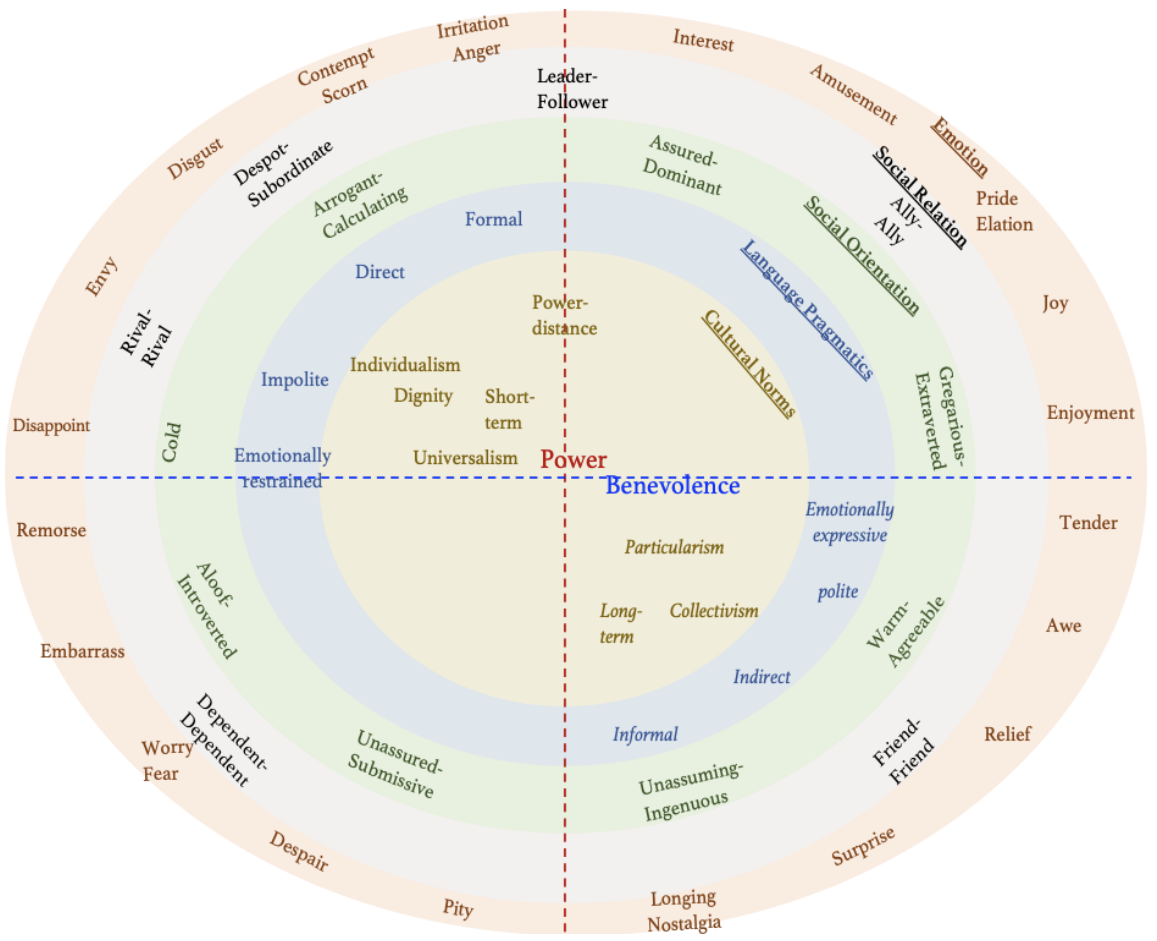
\includegraphics[width=0.75\textwidth]{./analysis/circumplex.png}
    \caption{Circumplex Theory Model}
    \label{fig:circumplex}
\end{figure}

I worked with Professor Colin Wayne Leach, Professor of Psychology \& Africana Studies from Barnard College to develop the social orientation tagging scheme and instructions. We engaged Yanda Chen, Yukun Huang, and 2 students from UIUC to label 8 videos using social orientation tags. Precision and recall results (as measured by our own implementation of LDC's scoring methodology) are presented in Table \ref{tab:social_orientation_annotation_results}.

\begin{table}[H]
    \centering
    \begin{tabular}{lll}
    \toprule
    Annotator & Precision & Recall \\
    \midrule
    Yanda Chen \& Yukun Huang & 0.53 & 0.47 \\
    UIUC Student 1 & 0.29 & 0.20 \\
    UIUC Student 2 & 0.50 & 0.20 \\
    \textit{Annotator Average} & \textit{\textbf{0.44}} & \textit{0.29} \\
    \midrule
    Best Mini-Eval System (video) & 0.05 & \textbf{0.77} \\
    \bottomrule
    \end{tabular}
    \caption{Social Orientation Annotation Results}
    \label{tab:social_orientation_annotation_results}
\end{table}

In particular, the prediction rule for this exercise was simple: treat all human annotations as change point annotations. In other words, whenever a person annotated a social orientation tag we treat it as a change point and compare to the ground truth LDC data. We see that this approach has relatively high precision compared to our best performing system from Fall 2022 on video data. This was an encouraging result because it suggested that social orientation tags could be a useful feature for change point prediction and might provide novel signal relative to our existing systems. In contrast, recall was lower than our best performing system, which is unsurprising given the large number of predictions that our systems tend to make.\\
\\
The social orientation annotation exercise highlighted questions about the consistency of LDC's change point annotation scheme. Recall that change points are defined as moments that may impact the relationship between the speakers in a significant way. We found that at least 5 out of 19 ``false positives'' found by human annotators may indeed be change points. Figure \ref{fig:change_point} shows one such example. These observations spurred calls for a program-wide annotation exercise to measure inter-annotator agreement and provided concrete evidence of the need for this.

\begin{figure}[H]
    \centering
    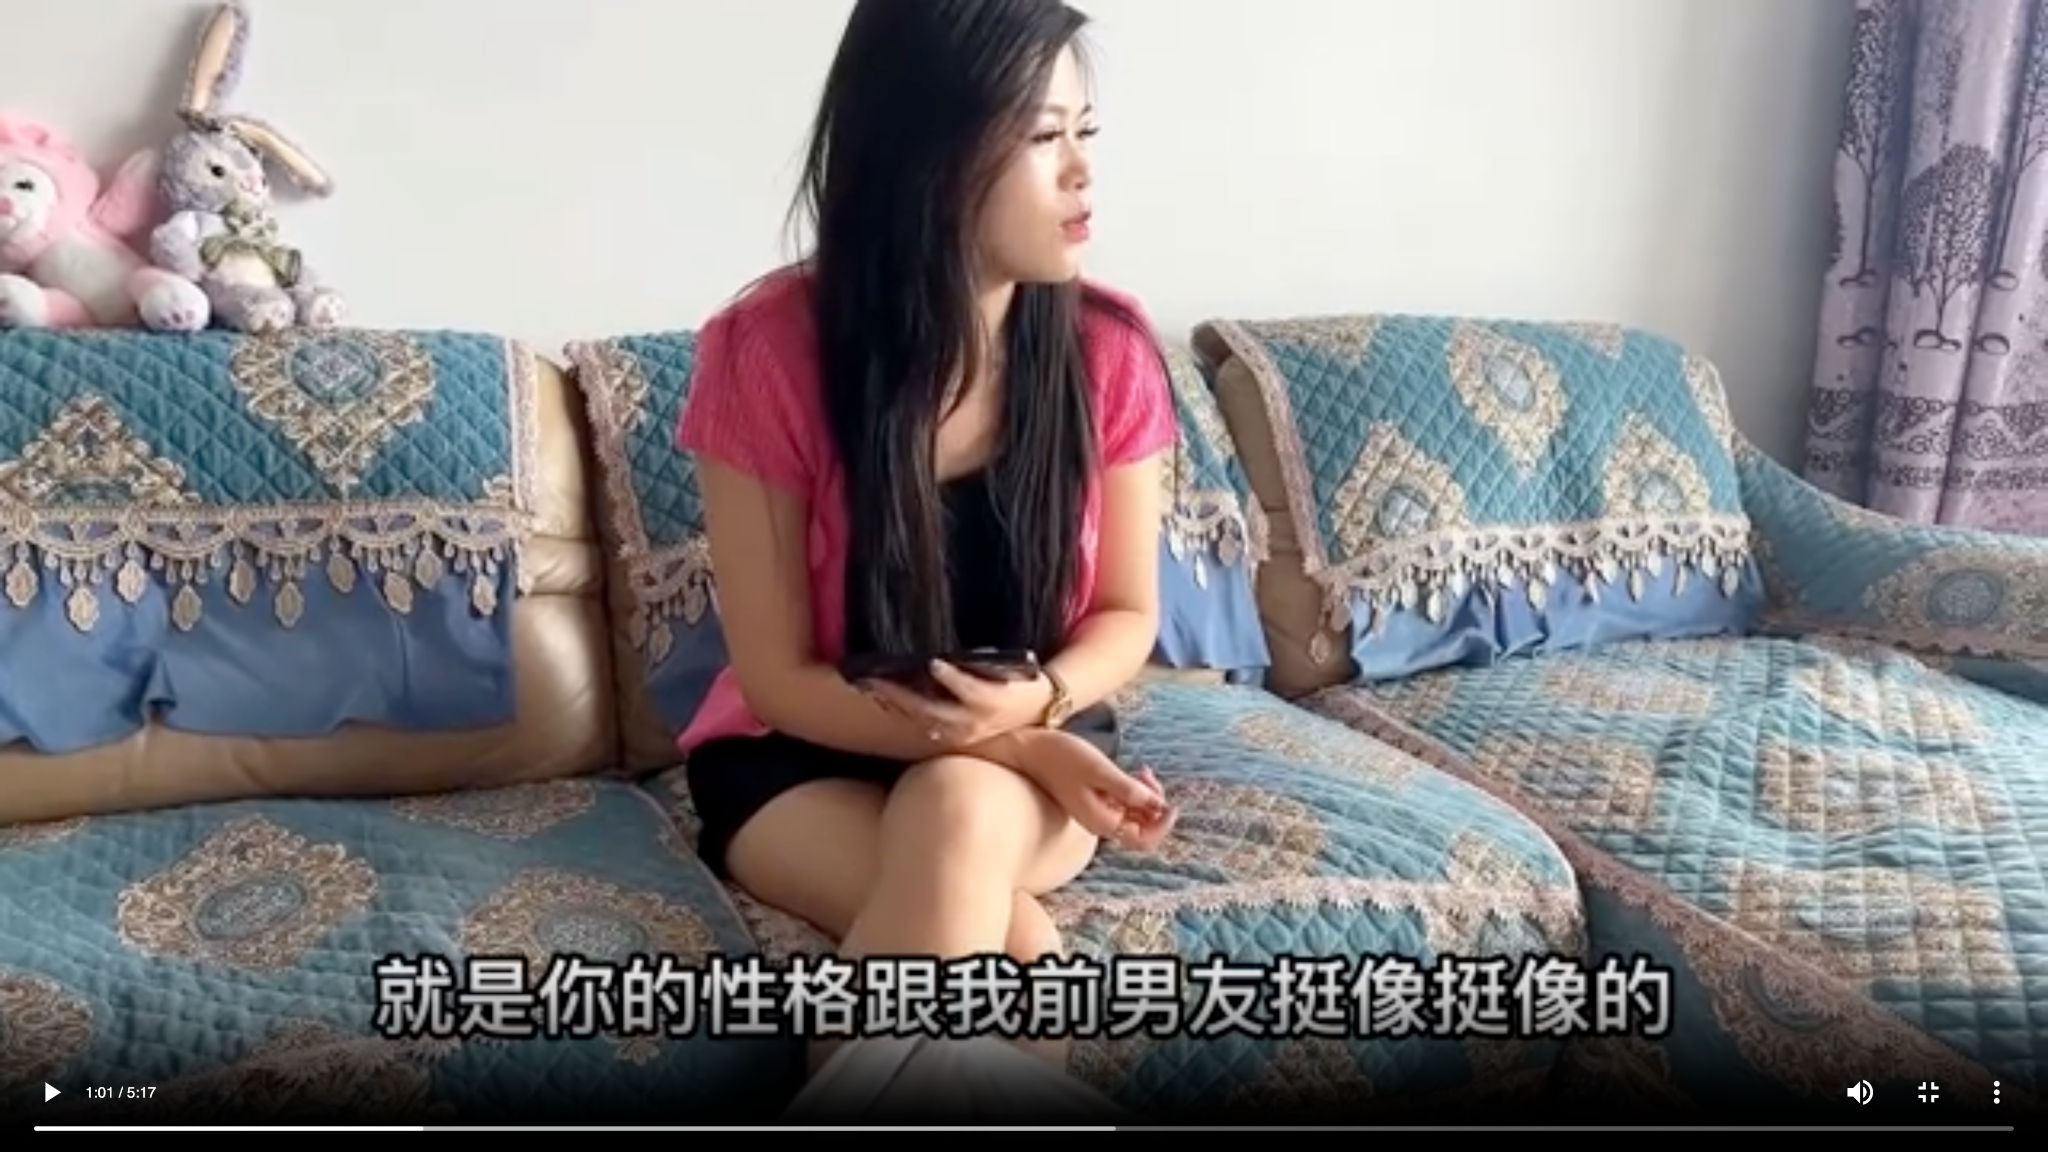
\includegraphics[width=0.75\textwidth]{./analysis/change_point.png}
    \caption{The speaker is quoted as saying, ``Your personality is very similar to my ex-boyfriend.'' which was a particularly low point in this conversation. This was not flagged as a change point by LDC.}
    \label{fig:change_point}
\end{figure}


\subsection{Scaling Social Orientation Annotation}
Encouraged by the results in the previous section, I used Generative Pre-Trained Transformer (GPT) models to scale up our labeled social orientation dataset so that we could include this feature into change point prediction systems. I developed a GPT prompt based on the annotation instructions developed for human annotators and prepared 311 text conversations for GPT annotation. These 311 conversations came from the BOLT Chinese SMS/Chat \cite{BOLT} corpus, which circumvents concerns about automatic speech recognition (ASR) quality issues because these are text conversations in the first place. This corpus also includes speaker information, which I hypothesized would be crucial for successfully annotating a social orientation dataset.\\
\\
I used \verb|gpt-3.5-turbo| via OpenAI's API to annotate the 311 conversations with a prompt that first describes the available tags, shows examples of the expected input and output format, and then asks the model to annotate the conversation. This prompt has been a work in progress and I've included the most recent iteration in the Appendix. A natural question is, how good are the social orientation annotations from GPT? I engaged Yanda Chen to evaluate one of the GPT annotated text conversations and he agreed with $\approx$50\% of the annotations. We then examined these annotations with respect valence (i.e. essentially treat the task as a binary classification task with positive and negative tags) and the model achieved an accuracy of 86\%.\\
\\
The NLP community is actively developing procedures for best exploiting large language models \cite{chen2023frugalgpt}. My experiences working with these models were as follows:
\begin{enumerate}
    \item Using a structured data format is crucial for getting good results. For example, I found that using Markdown over free-form text was crucial for being able to reliably parse GPT's annotations.
    \item GPT-4 does outperform GPT-3.5, when precision really matters. I found that GPT-4 and GPT-3.5 only agreed on about 26\% of labels for a sample conversation. Furthermore, GPT-4 can handle a larger context than GPT-3.5 (8,192 versus 4,097), which enables it to annotate an entire conversation at once rather than having to break it up into chunks, where chunking may introduce errors.
    \item However, GPT-4 is not truly production ready. Not only is GPT-4 30x more expensive than GPT-3.5 (\$0.06 / 1K tokens versus \$0.002 / 1K tokens), but its API is nearly unusable for long prompts (e.g. $>$4,000 tokens), which is unlikely to respond in a reasonable amount of time or at all\footnote{\url{https://community.openai.com/t/gpt-4-api-gateway-timeout-for-long-requests-but-billed-anyway/177214}}.
\end{enumerate}

\subsection{Social Orientation Classifier}
The next step was to develop a classifier that could label text utterances with social orientation tags. I trained an 8-way  XLM-RoBERTa classification model \cite{xlmr} that achieved 41\% accuracy and 57\% accuracy with respect to valence. Figure \ref{fig:confusion_matrix} shows a confusion matrix for the classifier.

\begin{figure}[H]
    \centering
    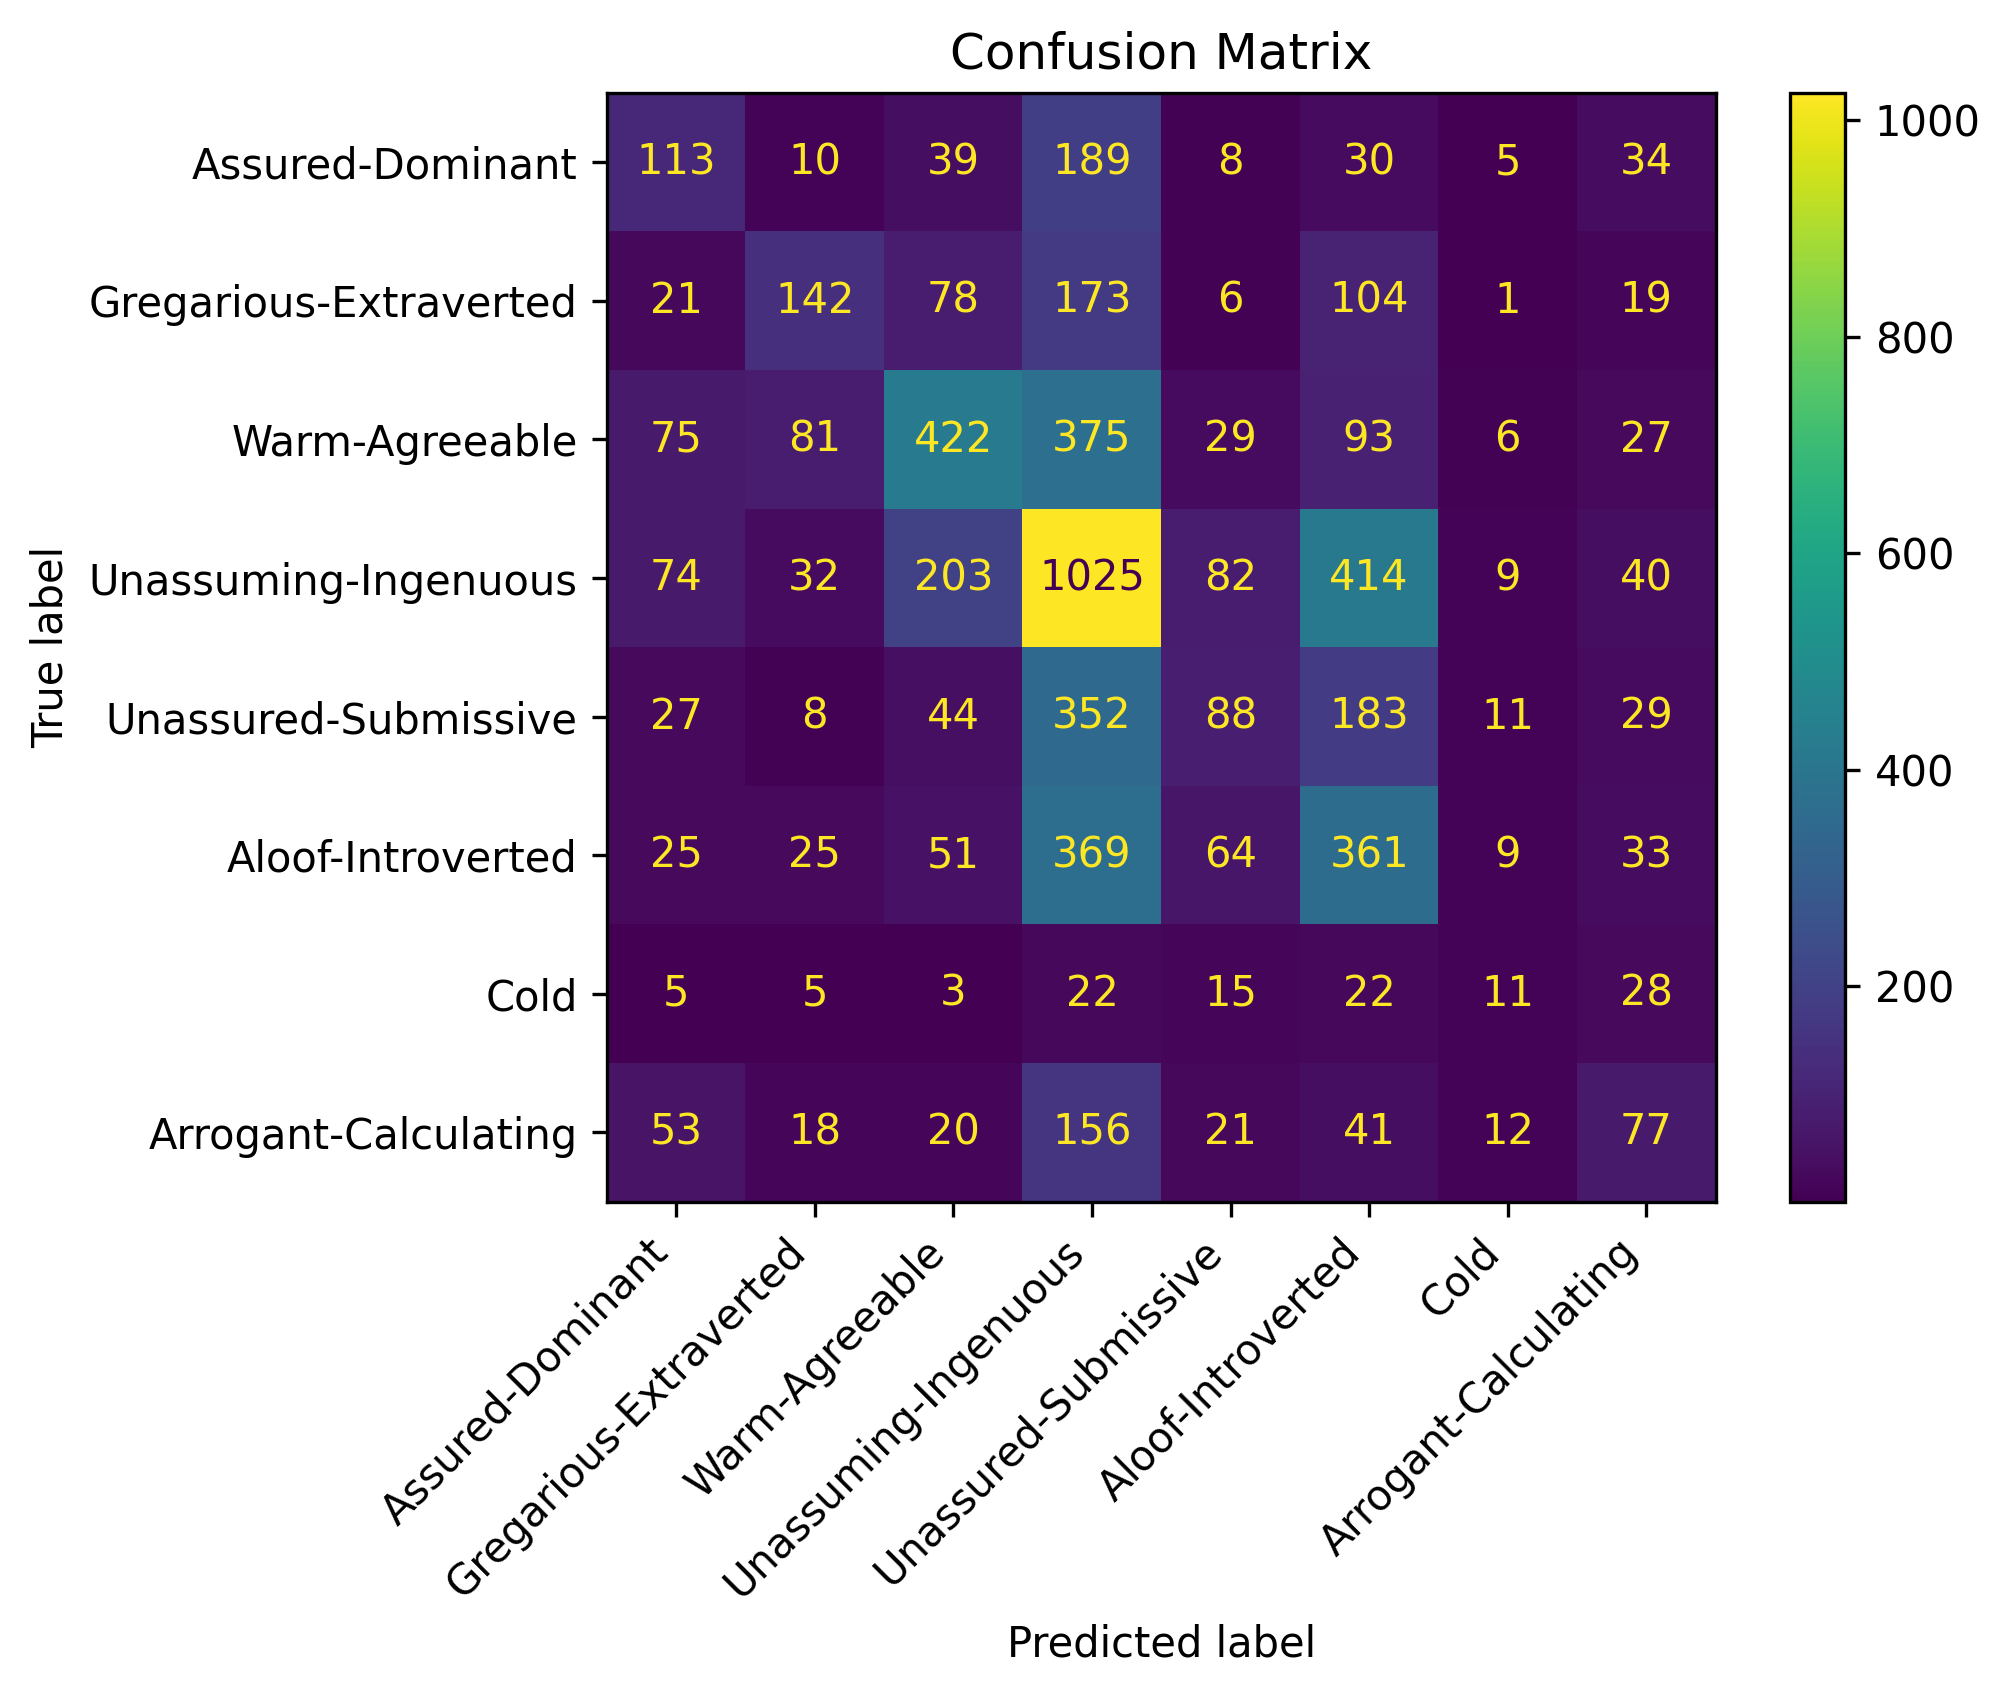
\includegraphics[width=0.75\textwidth]{./analysis/confusion.png}
    \caption{Confusion matrix for the Social Orientation classifier.}
    \label{fig:confusion_matrix}
\end{figure}

We note that the model predicts \verb|Unassuming-Ingenuous| a lot, which is a result of the class imbalance in the training dataset. We also note that treating the task as binary and predicting valence is a much easier task than the full 8-way classification. For example, examining the last row of the confusion matrix, we see that \verb|Arrogant-Calculating| is often confused with \verb|Assured-Dominant| and \verb|Aloof-Introverted|, where all of these tags have a somewhat negative valence.

\subsection{Change Point Prediction}
The ultimate objective of TA1.3 is to produce systems capable of detecting change points in conversations. My final task was to develop text-based change point prediction systems that could be used for full evaluation 1. In short, I developed 11 system variants, several of which incorporated social orientation tags as a feature. The system using social orientation achieved a text-based AP score of 0.242, the best among all systems I developed, which is an improvement over last semester's best AP score of 0.20.

\subsubsection{Model Architecture}
The model is an XLM-RoBERTa classification model that predicts a binary outcome (\{change point, no change point\}) for a size $k$ window (e.g. 20) of utterances. The label for a window of utterances is 1 (i.e. a change point) if a change point occurs during any utterance in the size $k$ window. The window is labeled 0 (i.e. no change point) if no change point occurs in the window. The tunable hyperparameters for this system are:
\begin{enumerate}
    \item \textbf{Social orientation:} prepends utterances with their predicted social orientation tags
    \item \textbf{Impact scalar:} trains a model using a cross entropy loss function for the classification scheme described above and adds a mean-squared error (MSE) loss for predicting impact scalars in the range (1-5)
    \item \textbf{Window size:} adjusts the window size parameter to include more or fewer utterances
    \item \textbf{Triplet loss:} adds a triplet loss function in addition to the cross entropy loss to improve separability of positive/negative examples. In particular, this loss function pushes positive examples (i.e. change points) closer together and negative examples closer together in the encoded space and pushes apart the positive and negative classes.
    \item \textbf{Loss reweighting:} this exposes a scalar $\lambda \in \mathbb{R^{+}}$ that weights the positive class more heavily than the negative class in the cross entropy loss function to address class imbalance.
\end{enumerate}

\subsubsection{Results}

Table \ref{tab:change_point_systems} shows AP scores on the validation set for all system variants. We note that the best performing system is the one that uses social orientation tags as a feature. We also note that higher positive class weight helps overcome class imbalance and that the impact scalar MSE loss may help.

\begin{table}[H]
    \centering
    \begin{tabular}{llrrr}
\toprule
                                             model &    filtering &  text &  video &  audio \\
\midrule
                   change-point-social-orientation &       lowest & 0.242 &  0.040 &  0.021 \\
                      change-point-medium-reweight & most\_similar & 0.242 &  0.027 &  0.008 \\
                        change-point-impact-scalar & most\_similar & 0.211 &  0.024 &  0.023 \\
                                      change-point & most\_similar & 0.176 &  0.042 &  0.031 \\
                       change-point-class-reweight & most\_similar & 0.176 &  0.042 &  0.031 \\
          change-point-small-reweight-large-window & most\_similar & 0.169 &  0.027 &  0.018 \\
  change-point-impact-scalar-small-reweight-social &       lowest & 0.147 &  0.003 &  0.000 \\
                       change-point-light-reweight &      highest & 0.132 &  0.002 &  0.000 \\
                        change-point-high-reweight &      highest & 0.127 &  0.024 &  0.019 \\
                         change-point-triplet-loss &      highest & 0.127 &  0.024 &  0.019 \\
change-point-light-reweight-high-window-impact-... &      highest & 0.090 &  0.001 &  0.000 \\
\bottomrule
\end{tabular}

    \caption{AP scores for all change point prediction system variants on the internal validation set along with the filtering procedure that attained the score.}
    \label{tab:change_point_systems}
\end{table}

I also examined the predictions made by one of my systems for a single file. Recall that my labeling approach generates $k$ positive labels for every ground truth change point, which may actually help with class imbalance. Based on this labeling scheme, one might imagine that the model starts predicting the presence of a change point $k/2$ turns before the ground truth change point and makes a total of about $k$ positive predictions. This means that we should think carefully about how we translate these predictions into a final change point prediction. For example, we might take the first positive prediction in the window as the change point, or we might take the last positive prediction as the change point. Another approach is to use a 1D convolution with weights the all 1s vector $\mathbbm{1}^k$, which sums up all the predicted probabilities in a sliding window of length $k$ and then set a threshold, such that whenever the sum of the probabilities in the window exceeds the threshold, we predict a change point. Figure \ref{fig:change_point_predictions} shows what this looks like for a single file.

\begin{figure}[H]
    \centering
    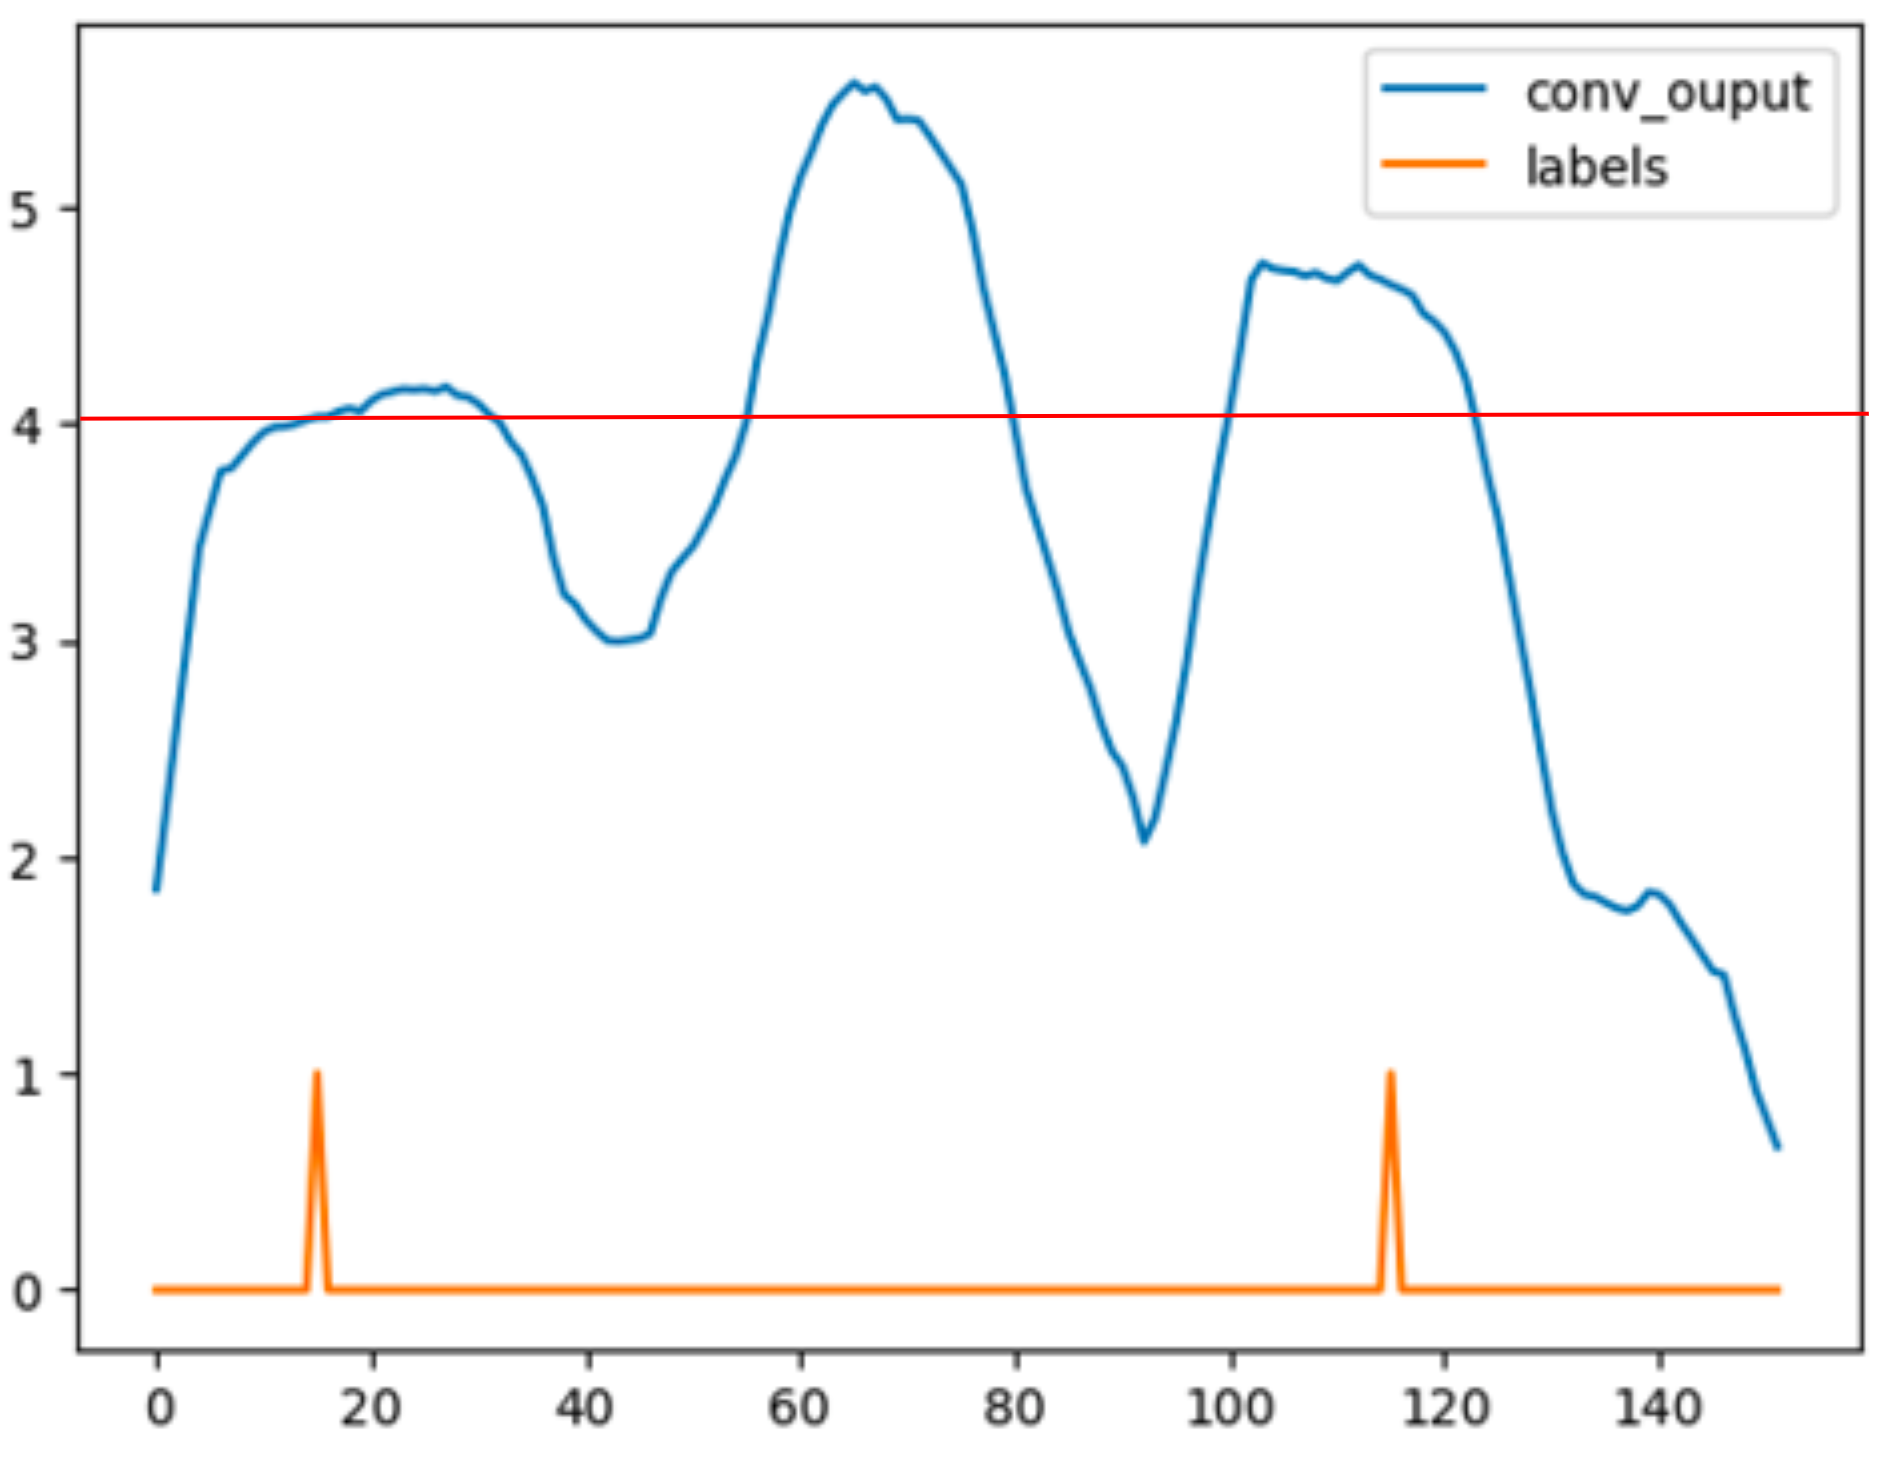
\includegraphics[width=0.75\textwidth]{./analysis/change_point_predictions.png}
    \caption{Change point predictions for a single file while applying a 1D convolution with weights $\mathbbm{1}^k$.}
    \label{fig:change_point_predictions}
\end{figure}

We see that if we use a threshold of about 4 and predict the peaks, we predict the 2 ground truth change points shown and have a third false positive prediction. Importantly, the point is to think creatively about how we translate our system predictions into change point predictions.

\subsection{Full Evaluation 1}
I produced predictions from  my system on the internal validation set, the test set, and the evaluation set, which contained data for over 6,000 videos. Full evaluation 1 was an enormous engineering challenge involving a lot of bookkeeping and compute power. I also note that I produced predictions for Tom Zollo's best performing system from Fall 2022.

\section{Integration \& Evaluation}
In the interest of brevity, I refer the reader to section \ref{sec:integration} for a summary of my contributions in the integration \& evaluation role. Here I provide a sketch of a potential application of our TA1.* systems, which DARPA may find useful for demonstrating the value of the program.

\subsection{Application}
One potential use case of our systems is to develop a meeting video annotation application that is integrated into Google Drive. It is very easy to record a Google Meets meeting (or meeting in any other video conference service) and the recording is stored in Google Drive. An application can then integrate with Google Drive and listen for newly uploaded videos or a user can provide a Google Drive link. A simple Streamlit\footnote{\url{https://streamlit.io/}} interface would be sufficient for this application (see Figure \ref{fig:streamlit_app} for a sample application). Our models are already hosted on AWS with clear API interfaces for change point, emotion, valence and arousal, and norms. The application would then make calls to our models with the user provided video, overlay our system predictions on the video (akin to the March PI meeting video), store the processed video on Google Drive, and then email the user a link to the annotated video. This application would be a simple way to demonstrate the value of our systems and would be a useful tool for post-hoc analysis of recorded meetings (e.g. for anyone that has to give a webinar and wants feedback on their performance).

\begin{figure}[H]
    \centering
    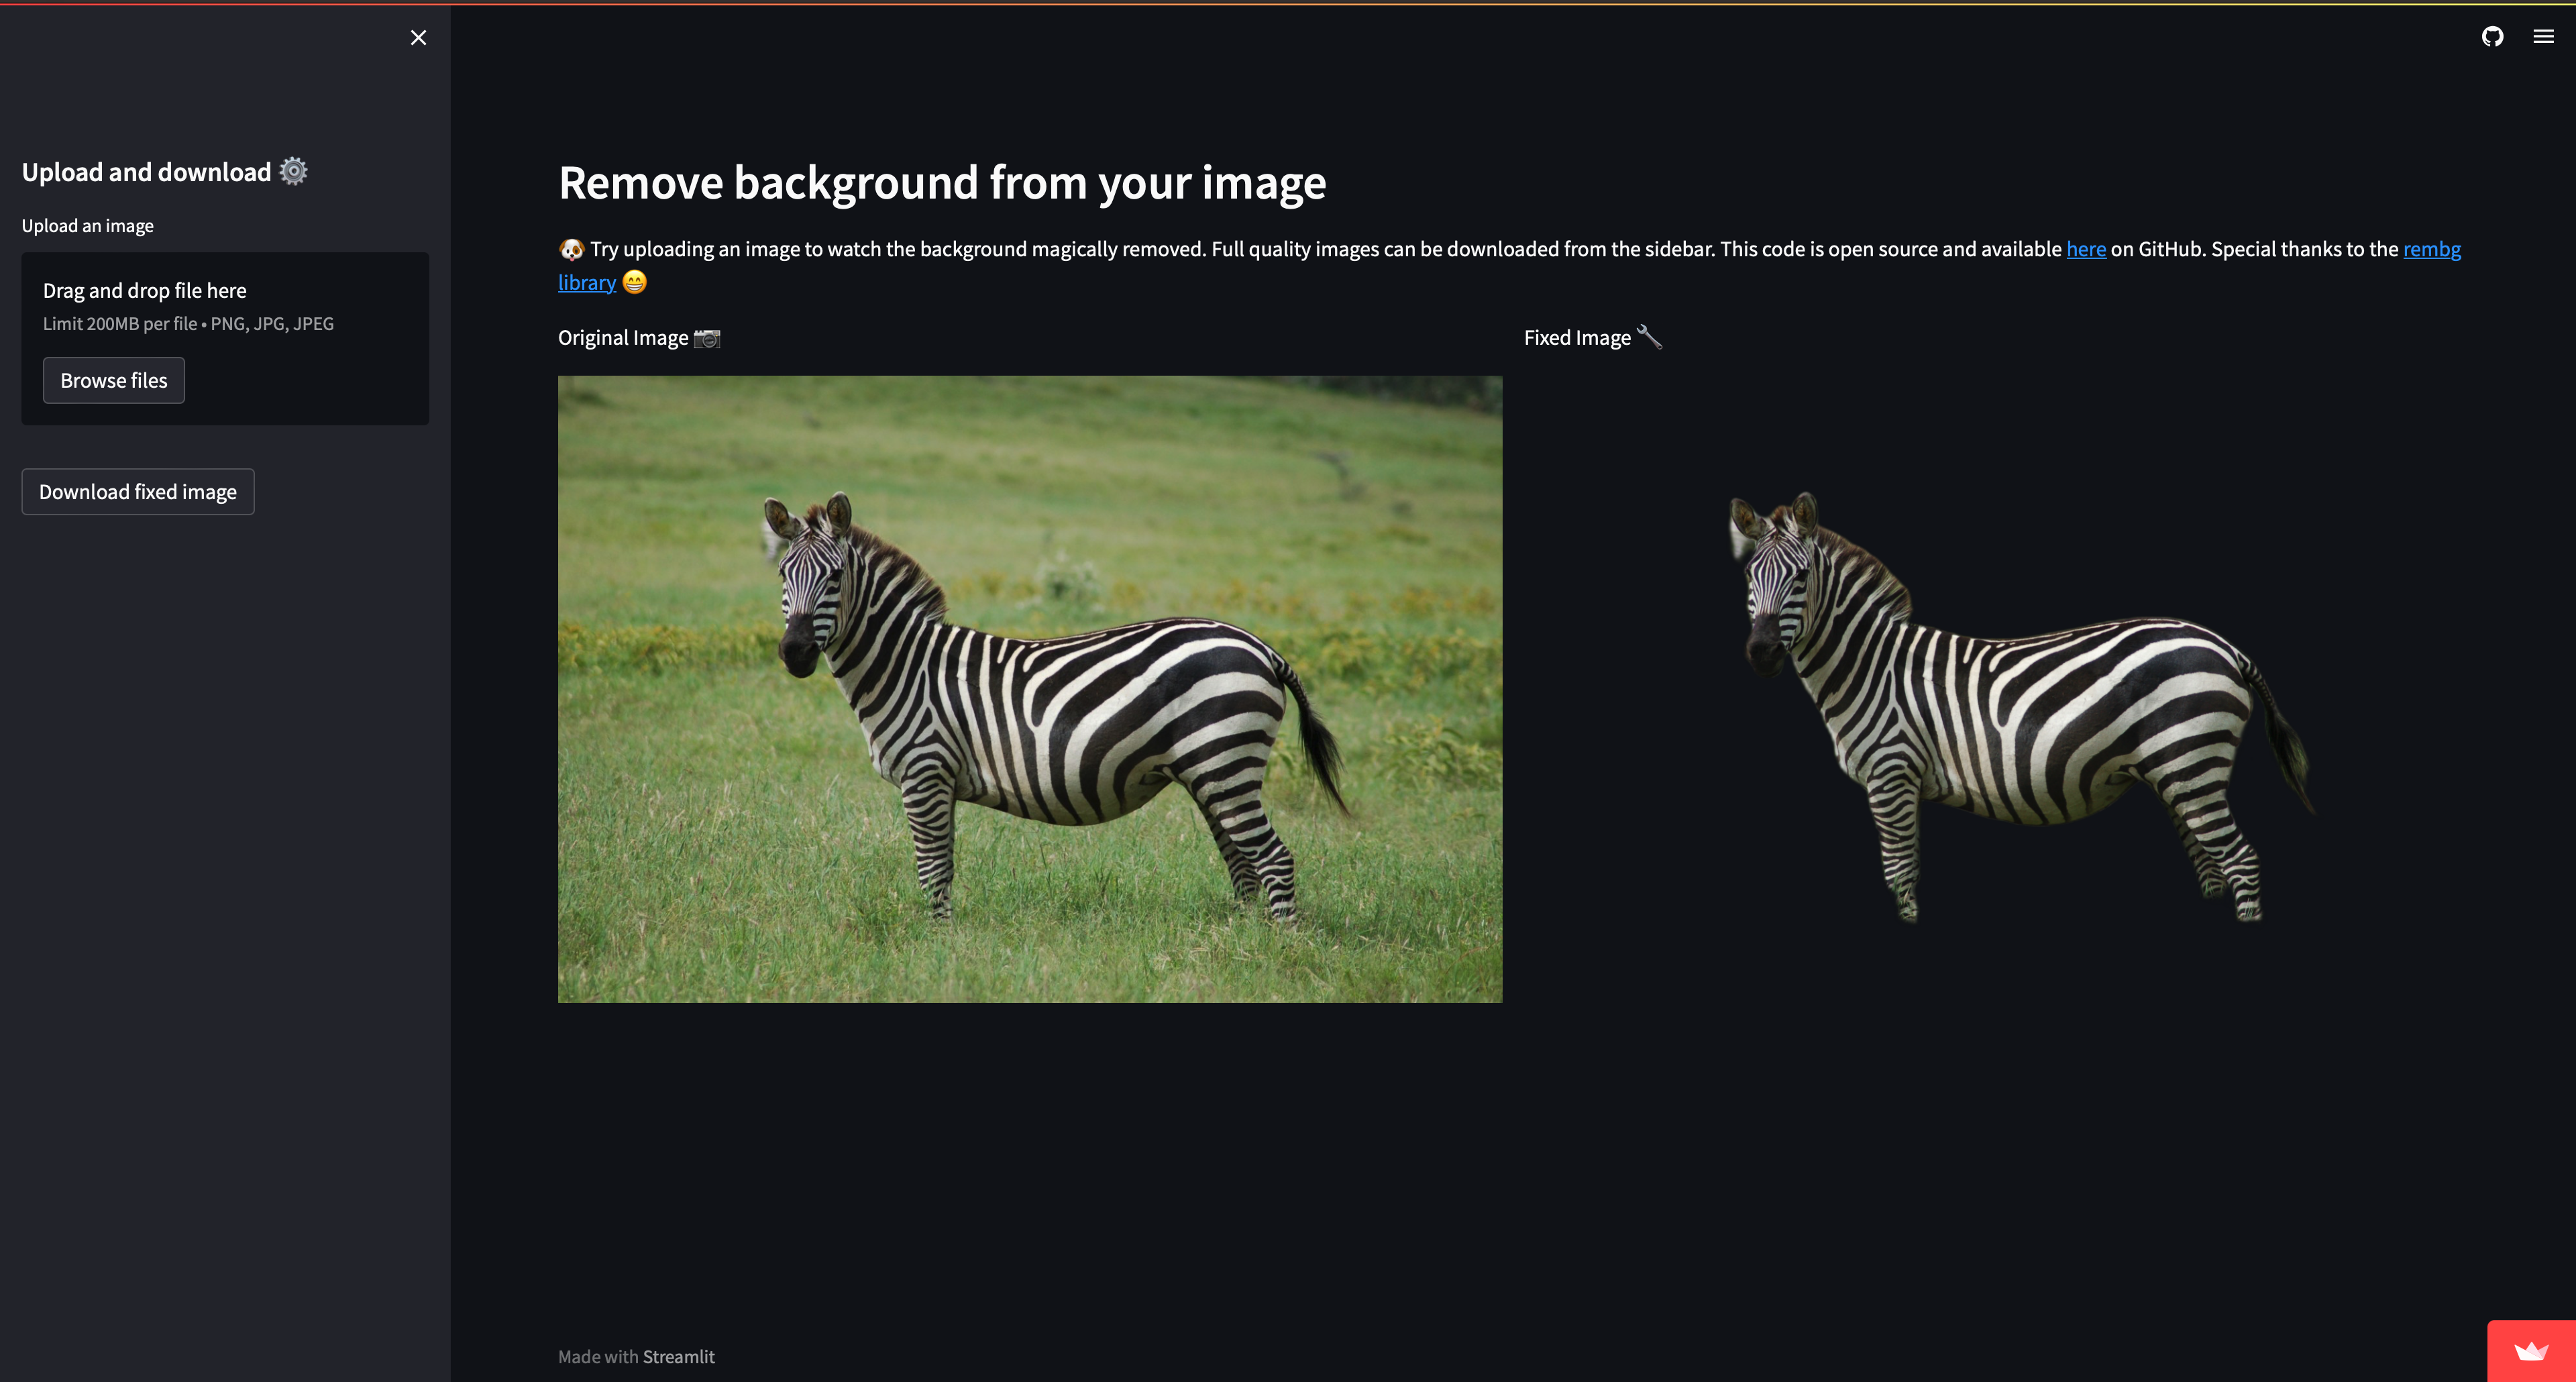
\includegraphics[width=0.75\textwidth]{./analysis/streamlit.png}
    \caption{A sample Streamlit application for removing the background from a user uploaded photo.}
    \label{fig:streamlit_app}
\end{figure}

\section{Next Steps}
All code for this project can be found at \url{https://github.com/ToddMorrill/charm}.

\subsection{Circumplex Theory, Social Orientation}
The following items can be refined to improve the performance of social orientation models:
\begin{enumerate}
    \item Refine the GPT prompt to use Markdown data formatting instead of free-form text to reduce the parsing errors. One can also experiment with using LDC metadata (e.g. modality, description, etc.) to contextualize the GPT prompt (see Table \ref{tab:metadata} for available metadata fields).
    \item Use GPT-4, when it's ready for production use, enabling longer context and higher quality predictions
    \item Incorporate loss weighting, a context window, and run a grid search
    \item Assess if the model is improving with more data and if so, obtain more labeled data from GPT
    \item Experiment with using GPT models for speaker diarization. Preliminary results show ~66\% accuracy on a sample video document. This may be useful for tracking the state of a conversation better and improving social orientation predictions.
\end{enumerate}

Beyond the above improvements, I spoke with Amith Ananthram about a potential research paper idea. The hypothesis for the paper is that social orientations tags are useful features for dialog tasks. Building on our positive results for the LDC change point dataset, we could examine if including social orientation tags as features improves performance for other corpora and tasks such as predicting successful outcomes for the Conversations Gone Awry dataset \cite{zhang2018conversations} or assessing the quality of a call center conversation.

\subsection{Change Point Prediction} 
The change point detection system would likely benefit from the following improvements:
% Implement early stopping against AP
% Retrain systems with GPT social orientation tags and with updated social orientation model predictions
% Experiment with using speaker information from text conversations or speaker diarization to better track the state of a conversation
% Experiment with new change point prediction procedures (e.g. convolutional models) (see next slide)
\begin{enumerate}
    \item Implement early stopping against AP
    \item Retrain systems with GPT social orientation tags and with updated social orientation model predictions
    \item Experiment with using speaker information from text conversations or speaker diarization to better track the state of a conversation
    \item Experiment with new change point prediction procedures (e.g. convolutional models).
\end{enumerate}

\subsection{Other Ideas for Change Point Prediction}
Here are a collection of other ideas that might be worth exploring for change point prediction:
% Experiment with using metadata provided by LDC for every available document (e.g. number of speakers, ages, setting, etc.)
% Determine if any of these metadata features are predictive of any of the tasks
% This can also be used to contextualize GPT annotations or model predictions. GPT may respond differently to different modalities if it had more information.
% Streaming approaches
% Consider context from earlier part of conversation (e.g. LSTM, etc.)
% Update some conversation state tracking representation
% Could be done with some sort of a trailing CLS representation from past transformer outputs
% Contrastive learning
% Predict cross-modal representations to develop a high quality encoder and TONS of unlabeled data
\begin{enumerate}
    \item Experiment with using metadata provided by LDC for every available document (e.g. number of speakers, ages, setting, etc.). See Table \ref{tab:metadata} for available metadata fields. These fields may also be useful for conditioning GPT predictions.
    \item Streaming approaches - consider context from earlier parts of a conversation, perhaps with an LSTM or other recurrent model. This could also be done with some sort of a trailing CLS representation from past transformer outputs.
    \item Contrastive learning - predict cross-modal representations to develop a high quality encoder using the copious amounts of unlabeled data we have access to.
\end{enumerate}

I will also note another research paper idea that I recently considered. The hypothesis of the paper is that metadata provides useful context for GPT models when silver labeling a dataset. While the hypothesis isn't particularly surprising, I suspect there is value in methodically quantifying the improvement in GPT predictions when using metadata. The paper might explore whether certain metadata fields are more useful than others. For example, for the IMDB sentiment classification dataset, we might examine how the inclusion of movie names, genres, plot synopsis, etc. improves the quality of GPT predictions. Similarly, in the context of social orientation tagging, we could include LDC provided document metadata and assess the improvement in the quality of the model's predictions. This research could be a good way to quantify the value of including metadata in prompts, which many people may have access to but may not be currently using.

\section{Acknowledgements}
I would like to thank Professor Kathleen McKeown for this incredible opportunity to work on this project. I would also like to thank Amith Ananthram and Yanda Chen for their guidance and support throughout the project. It's been a great opportunity to learn from both of them. Finally, I would like to thank Ivan Dewerpe, Harsha Vemulapati, Yi Fung, Revant Teotia, and Jeff (Zehui) Wu for their help with all things related to integration.

\printbibliography

\section{Appendix}
\subsection{Social Orientation Annotation GPT Prompt}
% multiline verbatim
\begin{lstlisting}
    Circumplex theory is a social psychology based theory that characterizes social interactions between speakers. The social orientation tagset includes: {Assured-Dominant, Gregarious-Extraverted, Warm-Agreeable, Unassuming-Ingenuous, Unassured-Submissive, Aloof-Introverted, Cold, Arrogant-Calculating}, which are defined below in more detail.

    Assured-Dominant - Demands to be the center of interest, demands attention, does most of the talking, speaks loudly, is firm, is self-confident, is forceful, is ambitious, is assertive, is persistent, is domineering, not self-conscious
    
    Gregarious-Extraverted - Feels comfortable around people, starts conversations, talks to a lot of different people, loves large groups, is friendly, is enthusiastic, is warm, is extraverted, is good-natured, is cheerful / happy, is pleasant, is outgoing, is approachable, is not shy, is "lively"
    
    Warm-Agreeable - is interested in people, reassures others, inquires about others' well-being, gets along well with others, is kind, is polite and courteous, is sympathetic, is respectful, is tender-hearted, is cooperative, is appreciative, is accommodating, is gentle, is charitable
    
    Unassuming-Ingenuous - Tolerates a lot from others, takes things as they come, tells the truth, thinks of others first, does not brag or boast, seldom stretches the truth, does not scheme or plot, is modest, is trustworthy, is unassuming, is honest, not self-centered, is sincere, not demanding, is straightforward
    
    Unassured-Submissive - Speaks softly, lets others finish what they are saying, dislikes being the center of attention, doubts themselves, not especially thorough, doesn't like to work too hard / will give up easily, is impractical, is timid, is inconsistent, is weak, is disorganized, is not authoritative, is a bit lazy, is not forceful
    
    Aloof-Introverted - Is quiet, especially around strangers, is a very private person, doesn't talk a lot / has little to say, doesn't smile much, doesn't reveal much about themselves, is not demonstrative (verbally or non-verbally), is distant, is shy, is impersonal, is introverted, is disinterested in others, is bashful, is not very social, is focused inward
    
    Cold - Believes people should fend for themselves, doesn't fall for sob-stories, is not interested in other people's problems, not warm toward others, is cruel, is ruthless, is cold-hearted, is hard-hearted, is unsympathetic, is uncharitable
    
    Arrogant-Calculating - Flaunts what they have, boasts and brags, will plot and scheme to get ahead, willing to exploit others for own benefit, is big-headed, is tricky, is boisterous, is conniving / calculating, is conceited, is crafty / cunning, is cocky, is manipulative of others
    ---
    In the following conversation, each row corresponds to an Utterance ID, a Speaker ID, and the Text spoken. For each utterance, assign a social orientation tag. Identify the utterance by its Utterance ID and Speaker ID. For example, here is the expected input and output format for a sample conversation.
    
    Input:
    | Utterance ID | Speaker ID | Text |
    | --- | --- | --- |
    | 1 | 1 | <Chinese content> |
    | 2 | 2 | <Chinese content> |
    | 3 | 1 | <Chinese content> |
    | 4 | 2 | <Chinese content> |
    | 5 | 2 | <Chinese content> |
    
    Output:
    | Utterance ID | Speaker ID | Label |
    | --- | --- | --- |
    | 1 | 1 | Aloof-Introverted |
    | 2 | 2 | Unassured-Submissive |
    | 3 | 1 | Warm-Agreeable |
    | 4 | 2 | Unassured-Submissive |
    | 5 | 2 | Cold |
    ---
    It's also possible that a speaker number is unknown for an utterance, in which case you should assign Speaker IDs to the utterances. Many conversations will have 2 speakers but some will have 3 or more. For example, here is the expected input and output format for such a conversation.
    
    Input:
    | Utterance ID | Speaker ID | Text |
    | --- | --- | --- |
    | 6 | unknown | <Chinese content> |
    | 7 | unknown | <Chinese content> |
    | 8 | unknown | <Chinese content> |
    | 9 | unknown | <Chinese content> |
    | 10 | unknown | <Chinese content> |
    
    Output:
    | Utterance ID | Speaker ID | Label |
    | --- | --- | --- |
    | 6 | 1 | Warm-Agreeable |
    | 7 | 2 | Warm-Agreeable |
    | 8 | 2 | Unassured-Submissive |
    | 9 | 2 | Unassured-Submissive |
    | 10 | 2 | Warm-Agreeable |
    ---
    Input:
\end{lstlisting}

% include metadata table with columns: Field Name, Description
% Field Name
% Description
% raw_synopsis
% brief free text description of the document content
% speaker_count
% the approximate speaker count. Options are 2, 3, 4+
% speaker_sex
% the sex of the speakers. Options are all_male, all_female, mix, unsure
% speaker_age
% the age of the speakers. Options are all_younger, all_middle, all_older, mix, unsure
% speaker_familiarity
% description of the relationship among speakers. Options are strangers, acquaintances, close, mix
% situation_type
% the conversation situation. Multiple values OK with each value delimited by comma. NOTE that the situation inventory may change in upcoming releases. Current options with brief explanation in parentheses: hangout (hanging out, family or social gathering) learning (learning situation, demo, tutorial, Q&A) business (business, business meeting, official meeting) debate (debate, argument, conflict) panel (panel, roundtable, group) negotiation (negotiation, problem solving) other (any other situation type)
% situation_other
% free text comment when 'other' situation type is selected * EMPTY_NA if 'other' is not selected in "situation_type" field
% formality_scalar
% formality scale. Options are 1, 2, 3, 4, 5 with 1 being least formal and 5 most formal. "EMPTY_TBD" is for judgments which will be updated in a subsequent release.
% minority_culture
% a true or false value indicating if the conversation contains speaker(s) from a culture other than Mainland China
\begin{table}[H]
\centering
\caption{Metadata fields available for all LDC annotated documents.}
\begin{tabular}{p{0.2\textwidth}p{0.8\textwidth}}
\toprule
\textbf{Field Name} & \textbf{Description} \\
\midrule
raw\_synopsis & brief free text description of the document content \\
\hline
speaker\_count & the approximate speaker count. Options are 2, 3, 4+\\
\hline
speaker\_sex & the sex of the speakers. Options are all\_male, all\_female, mix, unsure\\
\hline
speaker\_age & the age of the speakers. Options are all\_younger, all\_middle, all\_older, mix, unsure\\
\hline
speaker\_familiarity & description of the relationship among speakers. Options are strangers, acquaintances, close, mix\\
\hline
situation\_type & the conversation situation. Multiple values OK with each value delimited by comma. NOTE that the situation inventory may change in upcoming releases. Current options with brief explanation in parentheses: hangout (hanging out, family or social gathering) learning (learning situation, demo, tutorial, Q\&A) business (business, business meeting, official meeting) debate (debate, argument, conflict) panel (panel, roundtable, group) negotiation (negotiation, problem solving) other (any other situation type)\\
\hline
situation\_other & free text comment when `other' situation type is selected * EMPTY\_NA if `other' is not selected in ``situation\_type'' field\\
\hline
formality\_scalar & formality scale. Options are 1, 2, 3, 4, 5 with 1 being least formal and 5 most formal. ``EMPTY\_TBD'' is for judgments which will be updated in a subsequent release.\\
\hline
minority\_culture & a true or false value indicating if the conversation contains speaker(s) from a culture other than Mainland China\\
\end{tabular}
\label{tab:metadata}
\end{table}

\end{document}